\documentclass{article}
\usepackage{graphicx}
\usepackage{hyperref}

\title{TP Calcul Numérique}
\author{Nicolas BOUTON}

\begin{document}

\maketitle

\section*{Cours}

\subsection*{Notations}

\begin{itemize}
\item \textbf{SAXPY} : Scalar a fois X plus Y
\item \textbf{GAXPY} : General matrix A fois X plus Y
\item \textbf{DSL} : Domain Specific Language
\item \textbf{NNZ} : Number of Non Zero
\end{itemize}

\section*{Exercice 2}

Nous remarquons 3 chose :

\begin{itemize}
\item Augmentation du conditionnement avec la taille
\item Il faut considéré l'erreur arrière entaché du conditionnement
  pour avoir une approximation des résultats
\item Nous manipulons des algorithmes avec certaines complexité qui
  peuvent être algorithmique ou bien de mémoire
\end{itemize}

\underline{Graphiques :} \newline

Pour l'erreur relative avant :

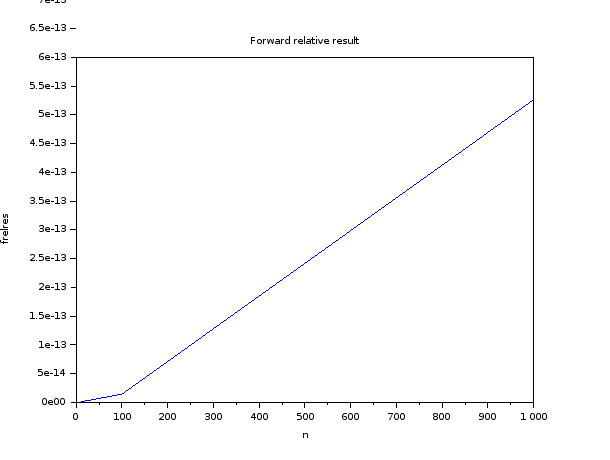
\includegraphics[scale=0.5]{img/frelres.png}


Pour l'erreur relative arrière :

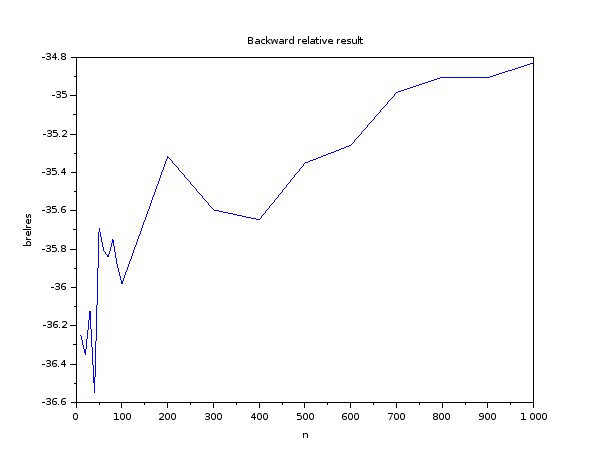
\includegraphics[scale=0.5]{img/brelres.png}

Pour le conditionnement de A :

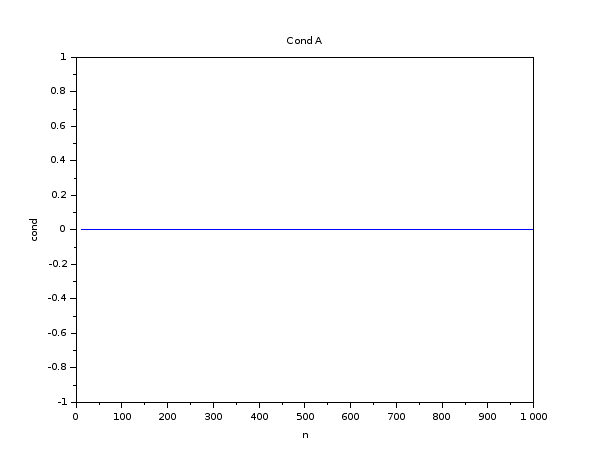
\includegraphics[scale=0.5]{img/capa.png}

Pour les bornes :

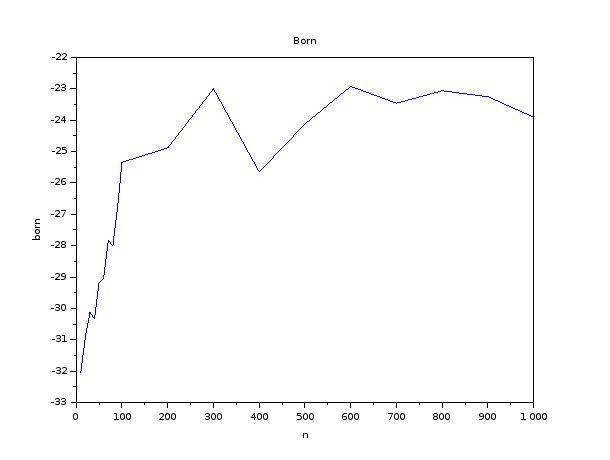
\includegraphics[scale=0.5]{img/born.png}

On voit que les erreurs relatives avant et arrières, ainsi que le
conditionnement de \textbf{A} et les bornes sont très sensible à la
taille de la matrice. De plus on peut apercevoir que c'est courbe
suivent une complexité logarithmique. En effet au début
l'augmentation de la taille entraîne une augmentation du résultat,
alors qu'a partir d'aune taille de \textbf{100 x 100} la courbe se
stabilise. \newline

Le code source se trouve dans \textbf{exo2.sci}.

\section*{Exercice 3}

Le produit \textbf{matrice x matrice} à une complexité cubique.
Nous remarquons dans un premier temps que l'appel au fonction de
\textbf{Scilab} pour des calculs \textbf{vecteur x vecteur} ou bien
\textbf{vecteur x matrice} au lieu de déroulé nous même les bloucles
est beaucoup plus performant. Il est d'autant plus performant si la
taille des matrices est grandes. \textbf{Scilab} appelle des noyaux de
calcul optimizé tel que \textbf{BLAS}. \newline

\underline{Graphiques :} \newline

Pour la fonction \textbf{matmat3b} :

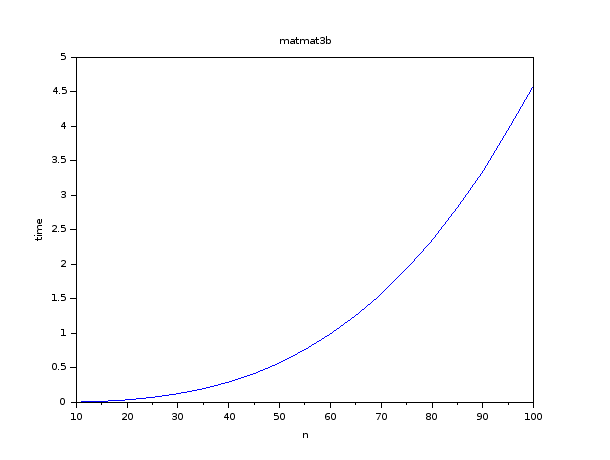
\includegraphics[scale=0.5]{img/matmat3b.png}

On voit que la fonction suit une complexité \textbf{cubique}, car
\textbf{Scilab} n'appelle pas \textbf{BLAS} à cause du fait que nous
avons déroulé 3 boucles. \newline

Pour la fonction \textbf{matmat2b} :

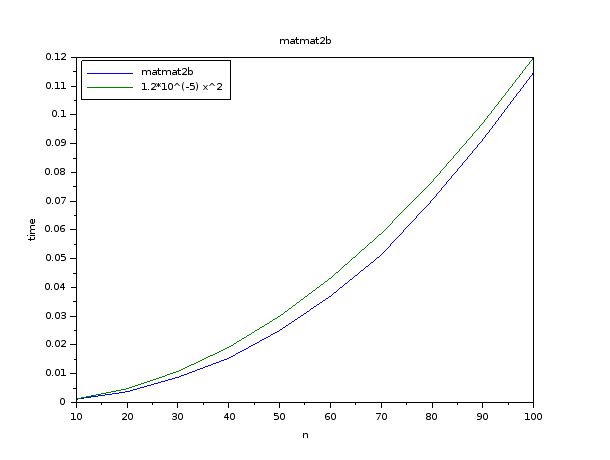
\includegraphics[scale=0.5]{img/matmat2b.png}

On voit que la fonction suit une complexité \textbf{quadratique}, car
\textbf{Scilab} appelle une fonction \textbf{vecteur x vecteur} de
\textbf{BLAS} ce qui réduit l'orde de 1, ce qui augmente la
rapidité. \newline

Pour la fonction \textbf{matmat1b} :

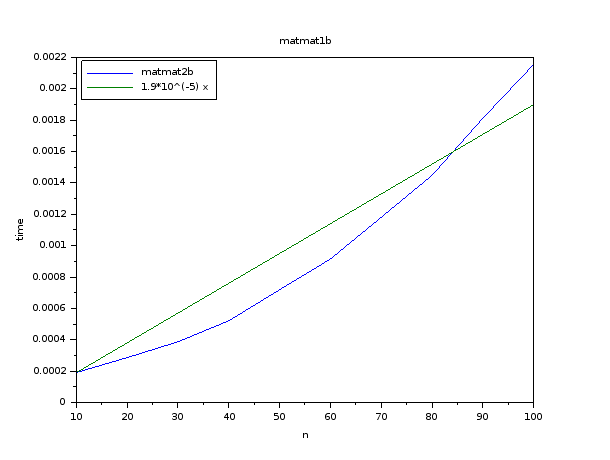
\includegraphics[scale=0.5]{img/matmat1b.png}

On voit que la fonction suit une complexité \textbf{linéaire}, car
\textbf{Scilab} appelle une fonction \textbf{vecteur x matrice} de
\textbf{BLAS} ce qui réduit l'ordre de 2, ce qui augmente la
rapidité. \newline

A l'avenir on appellera directement les \textbf{BLAS 3} c'est-à-dire
le produit \textbf{matrice x matrice} car le calcul est plus rapide.

\begin{itemize}
\item Le code des fonction se trouve dans \textbf{opmat.sci}.
\item Le code de test se trouve dans \textbf{exo3.sci}.
\end{itemize}

\section*{Exercice 4}

\underline{Graphiques :} \newline

Pour l'erreur relative avant pour les 2 matrices :

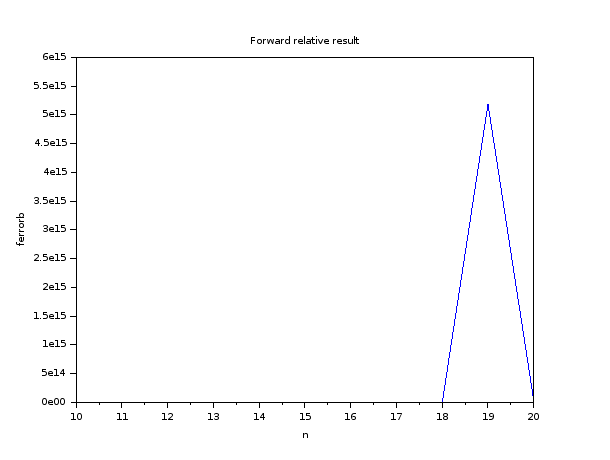
\includegraphics[scale=0.5]{img/ferrorb.png}

Pour l'erreur relative arrière pour les 2 matrices :

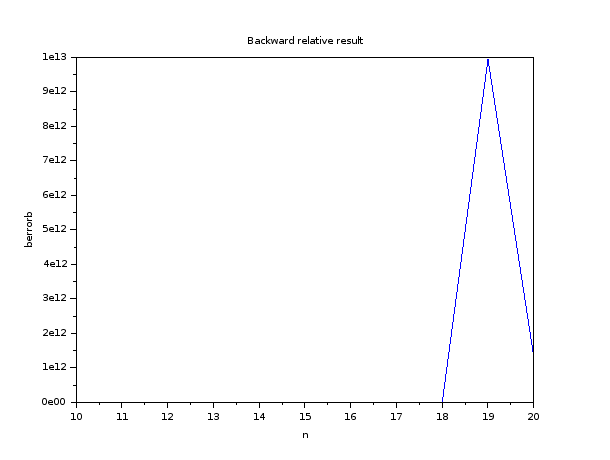
\includegraphics[scale=0.5]{img/berrorb.png}

Pour le conditionnement des 2 matrices :

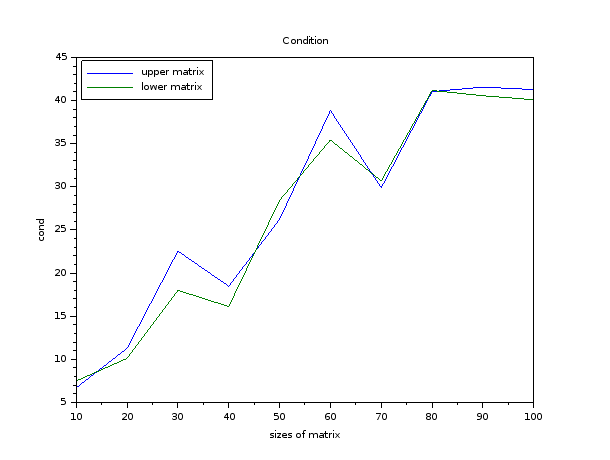
\includegraphics[scale=0.5]{img/condb.png}

On sait que l'erreur relative avant est borné avec la formule suivante
: \textbf{forward error $\le$ condition number x backward error} et
donc cela explique pourquoi nos errerus relatives avant se
dégrade très vite lorsque la taille augmente car le conditionnement
augmente très vite et les résultats sont entaché par le
conditionnement qui est quand à lui borné par la précision de la
machine qui est ici $10^{-16}$. \newline

Donc après une certaine taille l'erreur relative avant n'est plus une
erreur étant donné qu'il dépasse même le plus petit nombre entier
représentable qui est \textbf{1}. L'erreur est acceptable tant qu'elle
est inférieure à la précision machine qui est de $10^{-16}$. \newline

Donc pour les erreurs relatives arrières, elles sont acceptables car
elles sont inférieure à la précision machine qui est de
$10^{-16}$. \newline

\section*{Exercice 5}

Complexité de la méthode de \textbf{Gauss} :

\begin{itemize}
\item en temps  : $\frac{2}{3} n^3$
\item en espace : $O(n^2)$
\end{itemize}

\underline{Graphiques :} \newline

Pour les erreurs relatives :

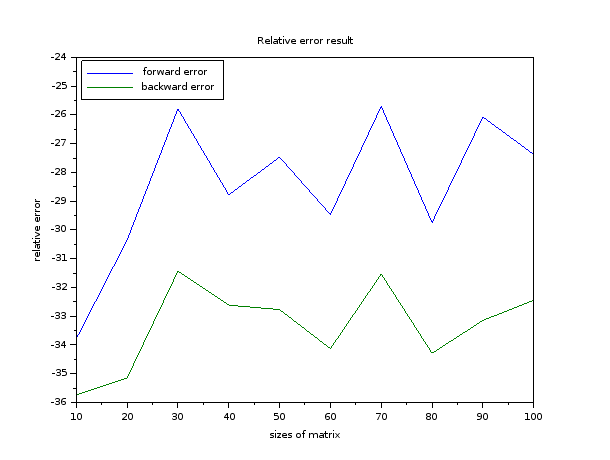
\includegraphics[scale=0.5]{img/gauss_error.png}

Les erreurs relatives avant et arrières sont acceptables car elles
sont inférieur à la précision machine qui est de $10^{-16}$. \newline

Et on a toujours l'erreur avant qui est plus élevé que l'erreur
arrière mais qui reste proportionnelle, c'est-à-dire que si l'une
baisse ou augmente l'autre fait de même étant donné qu'on a la
relation suivante qui borne l'erreur arrière : \newline
\textbf{forward error $\le$ condition number x backward
  error} \newline

Pour le conditionnement :

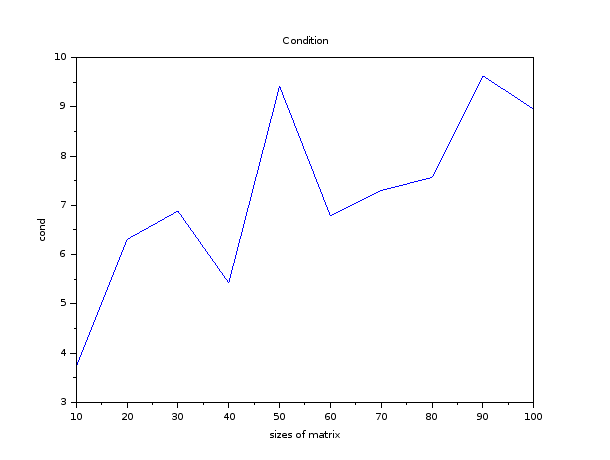
\includegraphics[scale=0.5]{img/gauss_cond.png}

Le conditionnement pour une taille de matrice \textbf{100 x 100} est
de $10^{10}$ ce qui peut donné un résultat avec au minimum une
précision de $10^{6}$ avec une précision machine de $10^{16}$.\newline

\section*{Exercice 6}

Complexité de la méthode \textbf{LU} :

\begin{itemize}
\item en temps  : $\frac{2}{3} n^3$ (mais 1 seul fois car indépendant
  du second menbre)
\item en espace : $O(n^2)$ (forme compact)
\end{itemize}

Remarques sur le pivot :

\begin{itemize}
\item éviter les pivots proches de zéro au début, ce qui implique
  d'utiliser des méthodes pour choisir les pivots
\item on priviliegera généralement le \textbf{pivot partiel} si on
  veut assurer une stabilité numérique, car le \textbf{pivot complet}
  est trop couteux et le gain en stabilité n'est pas assez bon
\end{itemize}


\section*{Annexe}

Dépot github : \url{https://github.com/Sholde/CN/tree/master/partie_2}

\end{document}
